\section{Results}\label{sec:results}
\subsection{A dispatch shortcut and residual trace context}\label{sec:dispatch}
\begin{table*}[t]\centering\small
\caption{Joint evaluation of the five live policies; 120 test fixtures per row, single host over loopback, synthetic tools. Sel.\ S/A: validation-selected size-only / adaptive attack (primary). Max: largest test count in the frozen suite (descriptive). GMM: label-free removal. Ref.: uniform six-class reference 20/120, or for shadow the realized pair-ambiguity floor (Table~\ref{tab:shadow-floor}). Bytes: whole-connection / call-window factors. Tokens include both planners. Goal and State are separate counts from this cohort; the state-control cohort (Supplement S1) has its own counts.}\label{tab:live-timing-main}
\setlength{\tabcolsep}{4pt}
\begin{tabularx}{\textwidth}{@{}lYrrrrrrr@{}}\toprule
Planner & Policy & Sel. S/A & Max & GMM & Ref. & Bytes$\times$ & Tokens$\times$ & Goal/State \\\midrule

Qwen3:8B & No cover & 117/117 & 117 & -- & 20 & 1.00/1.00 & 1.00 & 113/114 \\
Qwen3:8B & Immediate & 75/112 & 112 & 112 & 20 & 1.15/1.33 & 1.00 & 111/112 \\
Qwen3:8B & History, sequential & 76/93 & 99 & 53 & 20 & 1.15/1.32 & 1.00 & 112/113 \\
Qwen3:8B & History, concurrent & 66/99 & 99 & 38 & 20 & 1.15/1.33 & 1.00 & 111/112 \\
Qwen3:8B & Planner shadow & 54/54 & 70 & 34 & 70.5 & 1.31/1.68 & 2.01 & 112/113 \\
Llama3.1:8B & No cover & 110/110 & 112 & -- & 20 & 1.00/1.00 & 1.00 & 82/70 \\
Llama3.1:8B & Immediate & 80/108 & 108 & 108 & 20 & 1.13/1.27 & 1.01 & 83/67 \\
Llama3.1:8B & History, sequential & 82/104 & 104 & 14 & 20 & 1.13/1.26 & 1.01 & 84/67 \\
Llama3.1:8B & History, concurrent & 68/106 & 106 & 66 & 20 & 1.13/1.27 & 1.02 & 82/67 \\
Llama3.1:8B & Planner shadow & 64/64 & 64 & 43 & 70.5 & 1.35/1.71 & 1.99 & 82/67 \\
\bottomrule\end{tabularx}\end{table*}

\paragraph{Immediate cover exposes its short gap}
A label-free two-component mixture over training gaps selects the short-gap component for removal, and a classifier trained on no-cover traffic decodes the rest. With supplied call windows it recognizes 112/120 and 108/120 tasks, against selected size-only attacks at 75 and 80 (Table~\ref{tab:live-timing-main}). Both gains meet the replication rule after Holm correction ($p=1.9\times10^{-8}$ and $4.3\times10^{-6}$). Independent TCP reassembly matches all 773,450 TLS record types, lengths and counts, and packet-capture clocks reproduce both scores. The mixture flags 181/182 and 182/182 held-out immediate decoys with no false flags (Supplement S2.7). This directly supports the short-gap mechanism in the measured planner loop.

\paragraph{Sampled waits leave recognizable call context}
Sampling training gaps defeats the mixture: recognition falls to 53 and 14 (sequential) and 38 and 66 (concurrent). Context removal or joint decoding recognizes 93/120 and 104/120 sequential tasks against size-only attacks at 76 and 82, and 99/120 and 106/120 concurrent tasks against 66 and 68. Three comparisons survive Holm correction: Llama sequential ($p=.00078$) and both concurrent comparisons ($p<10^{-4}$); Qwen sequential does not ($p=.0559$).

These attacks use destinations, positions, sizes and timing relations. Direct timing-plus-size classification is weaker: Qwen scores 57 and 47 in the history arms, versus size-only LR's 61 and 52 (Supplement Table S6). Thus these policies leave useful trace context, but the history comparisons do not isolate timestamps. Because most controller schedules leave the requested action last, the last-destination rule alone still recognizes 75, 76 and 66 Qwen tasks in the three controller arms (Supplement Table S6). Whether the adaptive attacks' correct predictions concentrate on fixtures with an uncovered terminal action requires the retained per-fixture predictions and is not reported here. Sampled waits are minimums rather than matched conditional timing laws: Qwen's 40.5\,ms mean hold becomes 100.4\,ms sequential and 171.2\,ms concurrent at the observer (Table~\ref{tab:live-draws}).
\begin{table*}[t]\centering\small
\caption{Achieved history-based cover timing, all splits (455 cover calls per row). Means in seconds. An anchor gap is measured from the actual prior completed anchor call to cover record start. Sampled durations are minimum server holds, while achieved durations include record-level transport and scheduling.}
\label{tab:live-draws}
\begin{tabularx}{\textwidth}{@{}lYrrrr@{}}\toprule
Model & Arm & Drawn gap & Achieved anchor gap & Drawn hold & Achieved duration\\\midrule
Qwen & History seq. & 0.5198 & 0.5660 & 0.0405 & 0.1004\\
Qwen & History concurrent & 0.5198 & 0.5772 & 0.0405 & 0.1712\\
Llama & History seq. & 0.5865 & 0.6203 & 0.0768 & 0.1097\\
Llama & History concurrent & 0.5865 & 0.6204 & 0.0768 & 0.1234\\
\bottomrule\end{tabularx}
\end{table*}

Llama's sequential mixture deletes 477/634 honest calls while detecting only 64/182 cover calls, explaining its 14/120 score; joint decoding on the same traces reaches 104/120. A failed removal model therefore leaves a separate residual-recognition question.

\subsection{What survives without supplied call windows}\label{sec:noboundary}
We reanalyze all 3,000 episodes from complete encrypted connections, including setup and teardown. The attacker receives relative record times, directions, ciphertext lengths and destinations. Episode association remains supplied, but call endpoints, operation names, roles and HTTP stream assignments are removed. An idle-gap rule proposes events; raw-record classifiers skip this step. A training-only mixture removes short-gap events. The immediate-arm pair is the only primary test, and this suite lacks the stronger context and joint decoders of Section~\ref{sec:dispatch}.
\begin{table}[t]\centering\small
\caption{No supplied call boundaries; whole-episode association remains supplied. B/R: validation-selected idle-grid baseline and removal attacks (primary pair: immediate). Max: largest test count over both suites, including the exploratory protocol-aware eventizer designed after the idle-grid results were seen (descriptive). Counts out of 120; uniform reference 20.}\label{tab:no-call-main}
\setlength{\tabcolsep}{4pt}
\begin{tabularx}{\columnwidth}{@{}Yrrrr@{}}\toprule
 & \multicolumn{2}{c}{Qwen} & \multicolumn{2}{c}{Llama} \\\cmidrule(lr){2-3}\cmidrule(l){4-5}
Policy & B/R & Max & B/R & Max \\\midrule
No cover & 115/109 & 117 & 108/101 & 112 \\
Immediate & 80/69 & 91 & 90/86 & 97 \\
History, sequential & 73/74 & 75 & 88/56 & 93 \\
History, concurrent & 56/61 & 62 & 78/62 & 88 \\
Planner shadow & 69/65 & 73 & 69/56 & 69 \\
\bottomrule\end{tabularx}\end{table}

Selected removal recognizes 69/120 and 86/120 tasks against baselines of 80 and 90: paired differences $-9.2$ and $-3.3$ points (Holm $p=.025$ and $.54$). Thus the prespecified removal pipeline loses its advantage without supplied call windows. Its idle-gap events, however, match true calls with IoU-.5 F1 of 0.000 in eight of ten cells, including both immediate cells (Supplement Table S14), so removal operates on segments that do not correspond to calls. The negative result diagnoses this segmentation, not the protective value of withholding boundaries. A subsequent exploratory eventizer uses the padding quantum and MCP setup sequence. It changes Qwen's removal score from 68 to 91 and Llama's from 90 to 87, with event F1 .295 and .380 at IoU .5. It was designed after the first results and adds no confirmatory superiority claim.

Every arm retains above-chance recognition in the tested suite (Table~\ref{tab:no-call-main}). This supports residual recognition from associated encrypted connections and diagnoses this removal pipeline. Unknown-task discovery and strong context attacks on inferred events are separate questions. Unequal representations and suites prevent a causal comparison of boundary access.

\subsection{Recognition and work under planner shadows}\label{sec:shadow}
The strongest tested call-window attack, a size/destination RF, recognizes 70/120 Qwen and 64/120 Llama shadow tasks; validation-selected attacks score 54 and 64. Record-only maxima are 73 and 69 over 52 candidates, with selected attacks at 69 and 69. These are residuals of the complete shadow policy.

The shadow uses 8.14 and 10.46 total tool calls per fixture against controller cover's 5.6 and 6.8, changes their composition to a complete task, and uses 2.01 and 1.99 times the model tokens. Real-chain time rises from 2.91/3.33\,s to 4.80/3.94\,s; call-window bytes rise 1.68/1.71 times. This quantifies the complete policy's trade-off. Unlike the controller arms, the shadow adds a second business action to every episode, which alone could lower terminal-destination attacks. Isolating online planner generation requires a controller replay with matched calls, composition and terminal coverage.

The ideal observer in Section~\ref{sec:floor} knows both candidate labels but no real-chain identity. With 21 matching pairs among 120 fixtures, its reference is 70.5/120. The measured counts are compatible with that reference, which neither bounds actual trace attacks nor proves role indistinguishability. The chain attack recovers the real chain exactly in only 29 and 32 fixtures. On the 99 different-label cases, aggregate RF counts bound task accuracy only to $[49,70]/99$ and $[43,64]/99$; this is not a direct role test. Cache histories and start-order strata motivate that separate analysis (Supplement S2.5--S2.6). The shadow equivalence family compares identical selected attacks and supplies no indistinguishability evidence.

\subsection{Business outcomes from the same runs}\label{sec:state}
The live study records goal, state and cost on the same executions as traffic. All cover runs on isolated clones. Goal/state counts stay within three fixtures of no cover (Table~\ref{tab:live-timing-main}); honest paths match no cover on 115/120 Qwen and 103/120 Llama shadow fixtures. Llama's baseline goal/state counts, 82/70 of 120, define a limited executor baseline rather than a production reliability target.

A separate state-control cohort tests whether these endpoints distinguish collateral effects. Proxy, read and hidden-isolated cover keep Qwen state correctness at 115--116/120. Deliberate live writes reduce it to 7/120 while 102/120 goals complete, including 95 with collateral errors. Llama has 3/120 intact and 73 of 76 completed tasks with collateral errors. Both integrity reductions survive Holm correction ($p=3.7\times10^{-32}$ and $3.0\times10^{-19}$; Supplement S1). These constructed cases demonstrate endpoint sensitivity; their separate counts estimate no production damage rate.

\subsection{A worked screening example}\label{sec:decision}
Table~\ref{tab:decision} uses illustrative tolerances chosen after measurement. It is a descriptive worksheet, not a validated deployment decision. All call-window controller maxima exceed 60\%; shadow's displayed count intervals straddle it. A decision study must fix selection and uncertainty procedures in advance and cover every mandatory outcome, including paired goal/state changes and costs.

The sample has limited resolution near 60\%. An attack performing exactly at the iid reference $7/12\approx.583$ needs about 3,400 fixtures before its 95\% Clopper--Pearson upper limit falls below 60\% (1,983/3,400 gives .5999); at the distinct-label reference of .5, 60/120 already gives .593. Neither calculation is a powered role-equivalence study. Distinct-label sampling changes the ideal reference and remains unmeasured.

Record-only history results come from a weaker suite and cannot establish protection relative to the call-window suite. Observed mean costs are below the worksheet budgets; complete joint uncertainty is unassessed. Figure~\ref{fig:frontier} shows the measured policy points; Table~\ref{tab:shadow-floor} gives the ideal label references separately.
\begin{table*}[t]\centering\footnotesize
\caption{Descriptive screening worksheet. Tolerances were chosen after measurement: recognition $\le60\%$, goal/state point differences at most 3/120 below no cover, model tokens $\le2.5\times$, call bytes $\le2\times$ and mean real-chain latency $\le2\times$. CW Max is the largest tested count with a nominal 95\% Clopper--Pearson count interval, not an interval for all-attacker performance or a prospectively selected attack. Goal/state and costs are descriptive. Above and unresolved refer only to the worksheet; no policy has a validated joint pass. RO Max uses the 76-candidate exploratory record-only suite; the observation representations and attack suites differ.}\label{tab:decision}
\setlength{\tabcolsep}{3pt}
\begin{tabularx}{\textwidth}{@{}llrrrrrrYY@{}}\toprule
Planner & Policy & CW Max [95\% CI] & RO Max & $\Delta$G/$\Delta$S & Tok.$\times$ & Bytes$\times$ & Lat.$\times$ & CW screening & RO screening \\\midrule
Qwen3:8B & Immediate & 112 [.87, .97] & 114 & $-2$/$-2$ & 1.00 & 1.33 & 1.23 & Above: inference & Above: inference \\
Qwen3:8B & History, sequential & 99 [.75, .89] & 99 & $-1$/$-1$ & 1.00 & 1.32 & 1.47 & Above: inference & Above: inference \\
Qwen3:8B & History, concurrent & 99 [.75, .89] & 95 & $-2$/$-2$ & 1.00 & 1.33 & 1.14 & Above: inference & Above: inference \\
Qwen3:8B & Planner shadow & 70 [.49, .67] & 73 & $-1$/$-1$ & 2.01 & 1.68 & 1.65 & Unresolved: inference & Unresolved: inference \\\midrule
Llama3.1:8B & Immediate & 108 [.83, .95] & 112 & $+1$/$-3$ & 1.01 & 1.27 & 0.88 & Above: inference & Above: inference \\
Llama3.1:8B & History, sequential & 104 [.79, .92] & 111 & $+2$/$-3$ & 1.01 & 1.26 & 1.15 & Above: inference & Above: inference \\
Llama3.1:8B & History, concurrent & 106 [.81, .94] & 112 & $0$/$-3$ & 1.02 & 1.27 & 0.84 & Above: inference & Above: inference \\
Llama3.1:8B & Planner shadow & 64 [.44, .63] & 69 & $0$/$-3$ & 1.99 & 1.71 & 1.18 & Unresolved; state at point limit & Unresolved: inference \\\bottomrule
\end{tabularx}\end{table*}

\begin{figure}[t]\centering
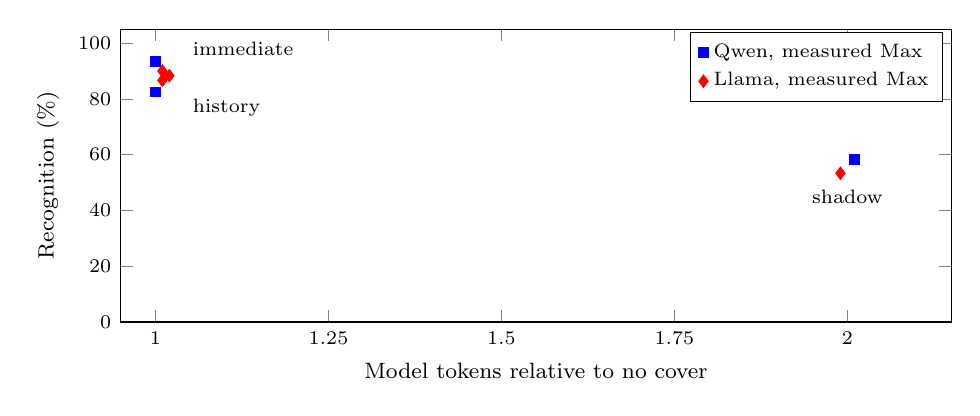
\begin{tikzpicture}
\begin{axis}[width=\columnwidth,height=5.3cm,xmin=0.95,xmax=2.15,ymin=0,ymax=105,
 xlabel={Model tokens relative to no cover},ylabel={Recognition (\%)},
 xtick={1,1.25,1.5,1.75,2},ytick={0,20,40,60,80,100},
 legend style={font=\scriptsize,at={(0.99,0.99)},anchor=north east,cells={anchor=west}},
 tick label style={font=\scriptsize},label style={font=\footnotesize}]
\addplot[only marks,blue,mark=square*,mark size=1.7pt] coordinates {(1,93.33) (1,82.5) (1,82.5) (2.01,58.33)};
\addlegendentry{Qwen, measured Max}
\addplot[only marks,red,mark=diamond*,mark size=2.2pt] coordinates {(1.01,90) (1.01,86.67) (1.02,88.33) (1.99,53.33)};
\addlegendentry{Llama, measured Max}
\node[font=\scriptsize,anchor=west] at (axis cs:1.04,98) {immediate};
\node[font=\scriptsize,anchor=west] at (axis cs:1.04,77) {history};
\node[font=\scriptsize,anchor=north] at (axis cs:2,51) {shadow};
\end{axis}
\end{tikzpicture}
\caption{Measured recognition and model work for the four cover policies. Points are strongest tested call-window attacks; overlapping controller points retain their values. Shadow changes call count and composition as well as model work. Ideal candidate-label values are shown separately in Table~\ref{tab:shadow-floor}.}\label{fig:frontier}
\end{figure}

